\subsection{Smoothing Spatial Filters}
Udglatning af billeder bruges til støjreduktion. Bruges også til at fjerne mindre detaljer, for at trække større detaljer ud. Det er dog ikke altid en god ide. Eksempelvis vil kanter i billedet blive hvisket ud. 

Dette kan vi gøre forbi støj selvregel består af små hurtige ændringer i intensitet.

\begin{figure}[H]
	\centering
	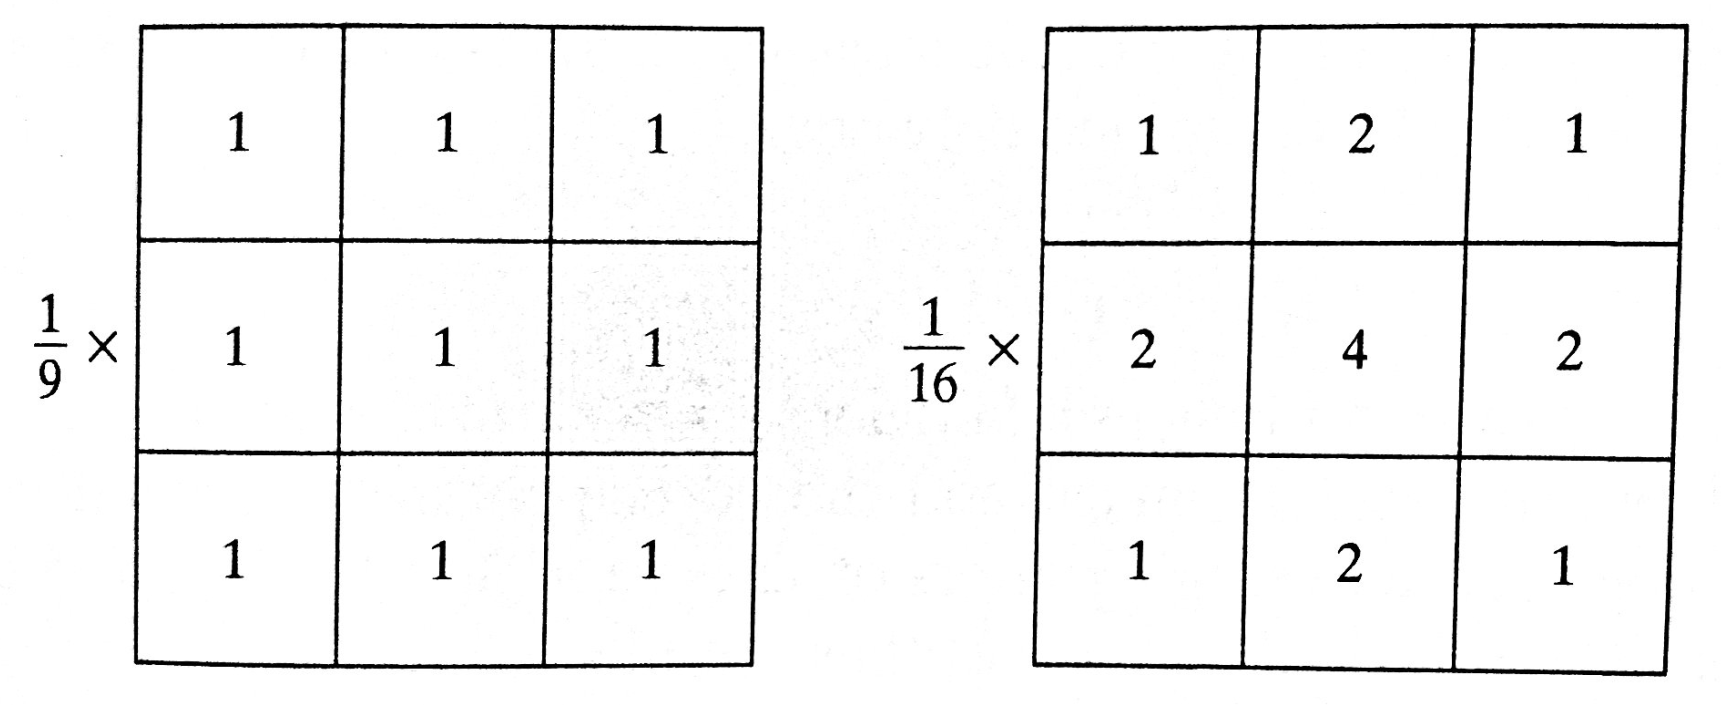
\includegraphics[width=0.7\linewidth]{figs/spm02/smoothing-filter}
	\caption{To filtre til udglatning. Det venstre kaldes også et box-filter, da alle tallene er ens.}
	\label{fig:smoothing-filter}
\end{figure}

Figur~\ref{fig:smoothing-filter} viser to filtre. Det andet filter kendes også som et: \textit{weighed average}, hvilket betyder at tallene ikke er ens. Udtrykket for et \textit{weighted average} filter er vist i Figur~\ref{fig:weightedfiltereq}. Dette står i modsætning til det andet filter i Figur~\ref{fig:smoothing-filter} som er et \textit{box-filter}.

\begin{figure}[H]
	\centering
	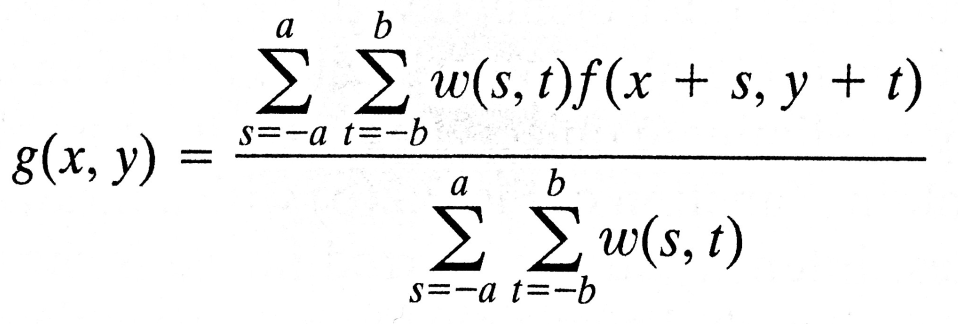
\includegraphics[width=0.55\linewidth]{figs/spm02/weightedfiltereq}
	\caption{Udtryk for et weighted filter.}
	\label{fig:weightedfiltereq}
\end{figure}

\subsubsection{Median filter}
Et median filter er det bedst kendte blandet de filtre som hører til kategorien af \textit{order-statistic (nonlinear) filter}. I stedet for at tage et gennemsnit af værdierne i ''nabolaget'' tager den median'en af tallene i området og sætte den midterste pixel værdi lig denne.

\begin{figure}[H]
	\centering
	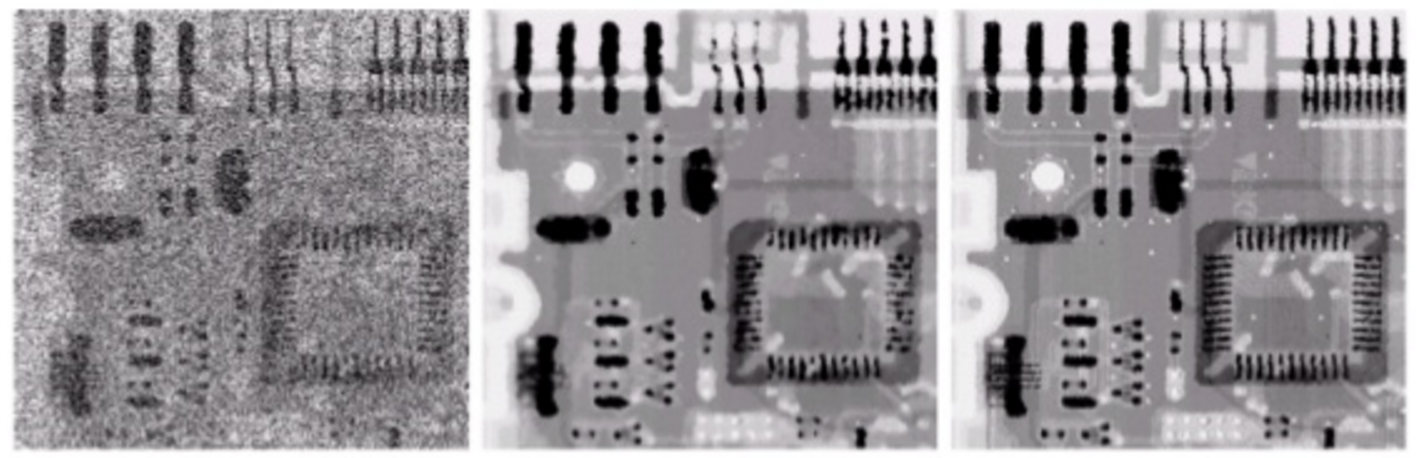
\includegraphics[width=0.9\linewidth]{figs/spm02/median-filter-salt-n-pepper}
	\caption{Et median filters effekt på salt-and-pepper støj.}
	\label{fig:median-filter-salt-n-pepper}
\end{figure}

Denne egenskab gør median filteret meget populært da det er rigtig godt til at fjerne støj uden at slørre billedet særlig meget. Især godt til \textit{impulse noise}, bedre kendt som salt-n-pepper støj, som vist på Figur.~\ref{fig:median-filter-salt-n-pepper}.
